\setcounter{section}{0}
\section{Логика и арифметика}

\subsection{Булевы функции, примеры. Двойственность.}
\textbf{Определение:} Булевая функция от $n$ аргументов - это функция $f: \{0,1\}^n\to \{0,1\}$. 

\textbf{Замечание:} Число всевозможных комбинаций аргументов, равно $2^n$, а количество булевых функций от $n$ аргументов равно $2^{2^n}$ (для каждой перестановки аргументов есть два значения функции - это 0 или 1).

\par \textbf{Определение:} Булевая функция $f^*$ называется двойственной булевой функции $f$, если она получена из $f$ инвверсией всех аргументов и самой функции, то есть \newline $f^*(x_1,\ldots,x_n)=\neg f(\neg x_1,\ldots,\neg x_n)$
\hfill \break

\begin{tabular}{| l | l | l | l | l | l | l | l | l |}
    \hline
    & & AND & OR & XOR & Импл. & Эквив. & Штрих Шеффера & Стрелка Пирса\\ 
    \hline
    $a$ & $b$ & $a\land b$ & $a\lor b$ & $a\oplus b$ & $a\rightarrow b$ & $a\Leftrightarrow b$ & $a\;|\;b$ & $a\downarrow b$\\ 
    \hline
    0 & 0 & 0 & 0 & 0 & 1 & 1 & 1 & 1\\
    0 & 1 & 0 & 1 & 1 & 1 & 0 & 1 & 0\\
    1 & 0 & 0 & 1 & 1 & 0 & 0 & 1 & 0\\
    1 & 1 & 1 & 1 & 0 & 1 & 1 & 0 & 0\\
\hline
\end{tabular}
\subsection{Классы булевых функций}
\begin{itemize}
    \item Класс $T_0$ функций, сохраняющих 0:
    $f \in T_{0}$, если $f(0,\dots ,0)=0$
    \newline Принадлежат: $0,\; id,\; a\land b, \; a\lor b,\; a\oplus b$ 
    \newline Не принадлежат: $1, \; \neg a$ 
    
    \item Класс $T_1$ функций, сохраняющих 1:
    $f \in T_{1}$, если $f(1,\dots ,1)=1$
    \newline Принадлежат: $1,\; id,\; a\land b,\; a\lor b,\; a\rightarrow b,\; a\Leftrightarrow b$ 
    \newline Не принадлежат: $0,\; \neg a$ 
    
    \item Класс $M$ монотонных функций:
    $f \in M$, если $\forall i(a_{i}\leqslant b_{i})\Rightarrow f(a_{1},\dots ,a_{n})\leqslant f(b_{1},\dots ,b_{n})$
    \newline Принадлежат: $0,\; 1,\; id,\; a\land b,\; a\lor b,\;$ 
    \newline Не принадлежат: $\neg a, \; a\oplus b $ 
    
    \item Класс $S$ самодвойственных функций:
    $f \in S$, если $f(\overline {x_{1}},\dots ,\overline {x_{n}})=\overline {f(x_{1},\dots ,x_{n})}$
    \newline Принадлежат: $id,\; \neg a,\; (x\land y)\lor (x\land z)\lor (y\land z)$ 
    \newline Не принадлежат: $0, 1\; a\land b $ 
    
    \item Класс $L$ линейных функций:
    $f\in L$, если $f(x_{1},\dots ,x_{n})=a_{0}\oplus a_{1}x_{1}\oplus \dots \oplus a_{n}x_{n},a_{i}\in \{0,1\}$
    \newline Принадлежат: $0,\; 1,\; id,\; \neg a,\; a\Leftrightarrow b,\; a \oplus b$ 
    \newline Не принадлежат: $a\land b $ 
    
\end{itemize}

\subsection{Пропозициональные формулы, КНФ и ДНФ}
Построение формул:
\begin{enumerate}
    \item Переменная -- это формула
    \item $\phi$ -- формула $\Rightarrow \; \neg \phi$ -- формула
    \item $\phi,\psi$ -- формулы $\Rightarrow \; (\phi\lor\psi), (\phi\land\psi), (\phi\to\psi)$ -- формулы
\end{enumerate}
\textbf{Определение:} $[\phi](a_1,\dots,a_n)$ -- значение формулы на наборе $\bar a(a_1,\dots,a_n)$
\begin{enumerate}
    \item $[p_i](\bar a)=a_i$
    \item $[\neg \phi](\bar a)=neg([\phi](\bar a))$
    \item $[\phi \land \psi](\bar a)=and([\phi](\bar a), [\psi](\bar a))$ и аналогично с $or, impl$
\end{enumerate}

\textbf{Определение:} Литерал -- переменная/формула вида $\neg p$, где $p$ - переменная

\textbf{Определение:} Конъюнкт -- конъюнкция литералов ($\land$)

\textbf{Определение:} Дизъюнкт -- дизъюнкция литералов ($\lor$)

\textbf{Определение:} КНФ -- конъюнкция дизъюнктов - $f(x,y,z)=(x\lor y)\land(y \lor \neg z)$

\textbf{Определение:} ДНФ -- дизъюнкция конъюнктов - $f(x,y,z)=(x\land y)\lor(\neg y \land \neg z)$

\textbf{Определение:} Тавтология -- формула, истинная при всех значениях входящих в нее переменных. Например, $((p \land q) \to p)$. 

Важные тождества: 1) $a\lor\neg a \equiv 1 \quad$ 2) $a\land \neg a \equiv 0$
\hfill \break
\newline \noindent \textbf{СКНФ/СДНФ (Cовершенные):}
\begin{enumerate}
    \item в ней нет одинаковых простых дизъюнкций (у СКНФ) и конъюнкций (у СДНФ);
    \item каждая простая дизъюнкция (у СКНФ) и конъюнкция (у СДНФ) полная.
\end{enumerate}
Например, СКНФ: $f(x,y,z)=(x\lor\neg y\lor z)\land(x\lor y\lor\neg z)$

\textbf{Теорема:} Для любой булевой функции, не равной тождественной 1, $\exists$ СКНФ, ее задающая.

\textbf{Теорема:} Для любой булевой функции, не равной тождественному 0, $\exists$ СДНФ, ее задающая.

\subsection{Многочлены Жегалкина}

\textbf{Определение:} Многочленом Жегалкина называется полином с коэффициентами вида 0 и 1, где в качестве произведения берётся конъюнкция, а в качестве сложения исключающее или: $P=a_{000\dots000}\oplus a_{100…0}x_1\oplus a_{010\dots0}x_2\oplus\dots\oplus a_{00…01}x_n \oplus a_{110\dots0}x_1x_2\oplus\dots\oplus a_{00\dots011}x_{n-1}x_n\oplus\dots\oplus a_{11\dots1}x_1\dots x_n$
\par \textit{Базовые функции:} а) $\neg p = p \oplus 1$ \quad б) $p\lor q = p \oplus q \oplus pq$ \newline \hangindent=4.25cm в) $p\land q = pq$ \quad в) $p\to q = 1 \oplus p \oplus pq$

Вычитание и сложение по сути одно и то же, поскольку все вычисления проходят по mod 2.


\subsection{Аксиомы исчисления высказываний, modus ponens}
\textbf{Теорема (корректности):} Любая выводимая формула есть тавтология.

\textbf{Теорема (полноты):} Любая тавтология выводима.
\newline Одним из возможных вариантов (гильбертовской) аксиоматизации логики высказываний является следующая система аксиом:

$A_{1}:A\rightarrow (B\rightarrow A)$;

$A_{2}:(A\rightarrow (B\rightarrow C))\rightarrow ((A\rightarrow B)\rightarrow (A\rightarrow C))$;

$A_{3}:A\wedge B\rightarrow A$;

$A_{4}:A\wedge B\rightarrow B$;

$A_{5}:A\rightarrow (B\rightarrow (A\wedge B))$;

$A_{6}:A\rightarrow (A\vee B)$;

$A_{7}:B\rightarrow (A\vee B)$;

$A_{8}:(A\rightarrow C)\rightarrow ((B\rightarrow C)\rightarrow ((A\vee B)\rightarrow C))$;

$A_{9}:\neg A\rightarrow (A\rightarrow B)$;

$A_{{10}}:(A\rightarrow B)\rightarrow ((A\rightarrow \neg B)\rightarrow \neg A)$;

$A_{{11}}:A\vee \neg A$.

вместе с единственным правилом: $\frac{A \quad A\rightarrow B}{B}$ (Modus ponens). Эта запись означает, что если выведены формулы $A$ и $A \to B$, то можно вывести $B$.

\subsection{Логические выводы и выводимые формулы}
\textbf{Определение:} Вывод -- конечная последовательность формул, каждая из которых либо является аксиомой, либо получается из ранее встретившихся по правилам вывода.

\textbf{Определение:} Формула называется выводимой, если она встречается в некотором выводе. Утверждение о том, что формула $\phi$ выводима в исчислении высказываний (ИВ), записывается так: $\vdash \phi$. \newline 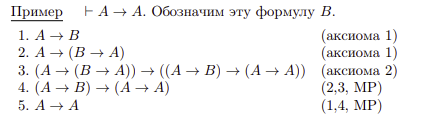
\includegraphics[width=0.6\linewidth]{images/1_definitions_mp}


\subsection{Резолюции}
\textbf{Определение:} Если $(A \lor x)$ и $(B \lor \neg x)$ одновременно истинны, то $(A \lor B)$ тоже истинно. Такое рассуждение называется правилом резолюции: $\frac{(A \lor x) \quad (B \lor \neg x)}{(A \lor B)}$

\textbf{Определение:} Дизъюнкт $(A \lor B)$ называется резольвентой дизъюнктов $(A \lor x)$ и $(B \lor \neg x)$.

\textbf{Замечание:} Резольвента дизъюнктов $x$ и $\neg x$ -- это пустой дизъюнкт, т.е. $\bot$.

\textbf{Метод резолюций для проверки КНФ на выполнимость:} Будем добавлять к набору дизъюнктов все возможные резольвенты. \newline Если в какой-то момент вывели $\bot$, то формула невыполнима. \newline Если нельзя применить правило резолюции так, чтобы получить новый дизъюнкт, а $\bot$ не выведен, то формула выполнима.

\subsection{Языки первого порядка}
\textbf{Определение:} Языки первого порядка — правила составления формул с кванторами, где кванторы берутся по отдельным объектам.
\newline \par \noindent Алфавит языка первого порядка:
\begin{itemize}
    \item Индивидная переменная (обычно буквы $x, y, z, t, u, v, w$) -- символ формального языка, служащий для обозначения произвольного элемента.
    \item Сигнатура $\sigma = \langle P_1,\ldots, P_k,f_1,\ldots,f_m \rangle$ -- набор предикатных и функциональных символов, обозначающих те или иные связи между объектами. 
    \begin{enumerate}
        \item Предикат валентности $N$ на множестве $A$ -- это функция $P:A^N\to \{0,1\}$ 
        \newline Предикатный символ — символ, обозначающий предикат. 
        \newline Например: $P^{(3)}, <^{(2)}, \subset ^{(2)}, Prime^{(1)}$
        
        \item Функция валентности $N$ на множестве $A$ -- это функция $f:A^N\to A$.
        \newline Функциональный символ — символ алфавита, обозначающий функцию.
        \newline Например: $f^{(3)}, +^{(2)}, \cap ^{(2)}, sin^{(1)}$
        \begin{itemize}
            \item[*] При этом символы валентности ноль -- это константы: $11, \pi, e, \O$
        \end{itemize}
    \end{enumerate}
    
    \item Символы логических операций: $\land, \lor, \neg, \to$
    \item Кванторы: $\forall, \exists$
    \item Служебные символы: скобки и запятые.
\end{itemize}

\textbf{Определение:} Терм -- строка, рекурсивно построенная по следующим правилам:
\begin{enumerate}
    \item Индивидная переменная есть терм;
    \item Функциональный символ валентности ноль (т.е. $f^{(0)}=const$) есть терм;
    \item Если $k > 0$, $f^{(k)}$ — функциональный символ валентности $k$, а $t_1,\ldots,t_k$ — термы, то $f^{(k)}(t_1,...,t_k)$ также терм.
\end{enumerate}

\textbf{Определение:} Атомарной формулой называется выражение вида $P^{(k)}(t_1,...,t_k)$ , где $k>0$, $t_1,\ldots,t_k$ — термы, а $P^{(k)}$ — предикатный символ валентности $k$.

\textbf{Определение:} Формулой (первого порядка) называется строка, рекурсивно построенная по следующим правилам:
\begin{enumerate}
    \item Атомарная формула является формулой;
    \item Если $\phi$ и $\psi$ являются формулами, то строки $(\phi \land \psi), (\phi \lor \psi), (\phi \to \psi), \neg\phi$ также являются формулами;
    \item Если $\phi$ является формулой, а $x$ — индивидная переменная, то $\exists x \phi$ и $\forall x \phi$ также являются формулами.
\end{enumerate}


\subsection{Интерпретация языка первого порядка, общезначимые формулы}
\textbf{Определение:} Пусть фиксирована некоторая сигнатура $\sigma$. Чтобы задать интерпретацию сигнатуры $\sigma$, необходимо:
\begin{itemize}
    \item указать некоторое непустое множество $M$, называемое носителем интерпретации;
    \item для каждого $k$-местного предикатного символа $P\in \sigma$ задана некоторая функция $[P]:M^k\to \{0,1\}$;
    \item для каждого $k$-местного функционального символа $f\in \sigma$ задана некоторая функция $[f]:M^k\to M$;
\end{itemize}

\textbf{Определение:} Оценкой переменных называется функция $\pi : Var \to M$, где $Var$ — множество индивидных переменных.
\begin{enumerate}
    \item $[\phi](\pi)$ -- значение формулы $\phi$ на оценке $\pi$
    \item $[t](\pi)$ -- значение терма $t$ на оценке $\pi$
\end{enumerate}

\textbf{Замечание:} Множество $Var$ заранее фиксировано, все термы и формулы строятся на его основе, а оценка
задаёт значения всех переменных из этого множества.
\newline \par Пусть фиксированы интерпретация $I$ и оценка $\pi$. Тогда для каждого терма $t$ должно возникнуть его значение, которое мы будем обозначать через $[t](\pi)$ (зависимость
от интерпретации в явном виде писать не будем, поскольку она не будет меняться в дальнейших определениях, а оценка будет). Поскольку терм строился рекурсивно, его
значение также будет определяться последовательно для всех шагов рекурсии.
\begin{itemize}
    \item[*] Если $t\eqcirc x$, где $x$ -- переменная, то $[t](\pi)=\pi(x)$
    \item[*] Если $t\eqcirc c$, где $c$ -- функциональный символ валентности 0, то $[t](\pi)=[c]$
    \item[*] Если $t\eqcirc f(t_1,\ldots,t_k)$, то $[t](\pi)=[f]([t_1](\pi),\ldots,[t_k](\pi))$
\end{itemize}
Значение формулы также определяется рекурсивно.
\begin{itemize}
    \item[*] Если $\phi\eqcirc P(t_1,\ldots,t_k)$ -- атомарная формула, то $[\phi](\pi)=[P]([t_1](\pi),\ldots,[t_k](\pi))$
    \item[*] Если $\phi\eqcirc \neg\psi$, то $[\phi](\pi)=not([\psi](\pi))$ 
    \item[*] Если $\phi\eqcirc \psi \lor\gamma$, то $[\phi](\pi)=or([\psi](\pi),[\gamma](\pi))$ (аналогично для $\land, \to$)
\end{itemize}

\textbf{Замечание:} Символы логических операций слева от знака равенства являются просто символами, а
справа мы обозначаем соответствующую булеву функцию.
\newline \par  Наконец, перейдём к самому интересному -- кванторам. Это единственный случай,
где изменяется не только формула, значение которой определяется, но и оценка.

\hfill \break
\begin{minipage}{0.6\textwidth}
  \begin{itemize}
    \item[*] Если $\phi\eqcirc \forall x \psi$, то $[\phi](\pi)=\land_{m\in M}[\psi](\pi_{x\to m})$
    \item[*] Если $\phi\eqcirc \exists x \psi$, то $[\phi](\pi)=\lor_{m\in M}[\psi](\pi_{x\to m})$
    \end{itemize}
\end{minipage}
\hfill
\begin{minipage}{0.4\textwidth}
    $\pi_{x\to m} (y)= 
    \begin{cases}
        \pi(y), \; y\neq x \\
        m, \; y==x
    \end{cases}$
\end{minipage}
$$
\land_{m\in M}Q_m=
    \begin{cases}
        1, \; \text{все }Q_m \text{ равны 1} \\
        0, \; \text{иначе}
    \end{cases}
    \qquad 
\lor_{m\in M}Q_m=
    \begin{cases}
        0, \; \text{все }Q_m \text{ равны 0} \\
        1, \; \text{иначе}
    \end{cases}
$$

\hfill \break
\textbf{Определение:} Общезначимая формула -- формула, истинная при любой интерпретации на любой оценке

\textit{Пример 1:} Для любой формулы $\phi$ формулы $\forall x\forall y\phi \to \forall y\forall x\phi$ и $\exists x\exists y\phi \to \exists y\exists x\phi$

\textit{Пример 2:} Для любой формулы $\phi$ формулы $\exists x\forall y\phi \to \forall y\exists x\phi$. Обратная импликация общезначима не всегда. Например, если некоторое блюдо попробовали все гости, то каждый гость попробовал хотя бы одно блюдо. Но если к каждому замку подходит некоторый ключ, это ещё не значит, что один из ключей подходит сразу ко всем замкам

\subsection{Свободные и связные вхождения переменных. Параметры формулы.}
\textbf{Определение:} Говорят, что переменные, от которых не зависят значения формул, связаны некоторым оператором ($\sum, \lim, \max$ или каким-нибудь ещё) и потому называются связанными, а остальные переменные свободны. Более корректно говорить не о связанных и свободных переменных, а о связанных и свободных вхождениях переменных.
\newline 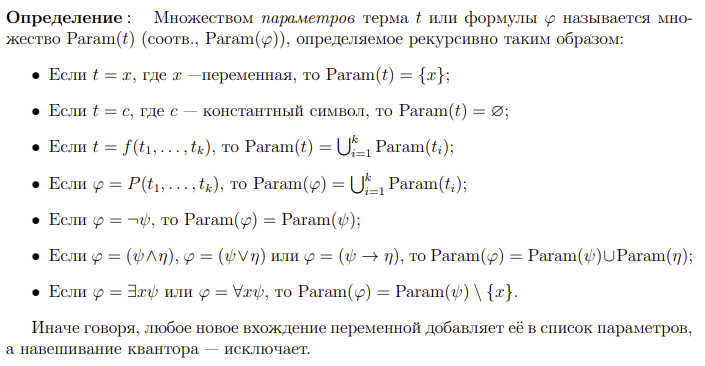
\includegraphics[width=0.9\linewidth]{images/1_definitions_param.png}

\subsection{Выразимость предиката или функции в данной интерпретации.}
Зафиксируем некоторую сигнатуру $\sigma$ и ее интерпретацию с носителем $M$.

\textbf{Определение:} Формула $\phi$ с параметрами $x_1,\ldots,x_m$ выражает предикат $P:M^m\to \{0,1\}$, если $\phi(a_1,\ldots,a_m)=1 \Leftrightarrow P(a_1,\ldots,a_m)=1$.

\textbf{Определение:} Функция $f : M^n \to M$ называется выразимой, если существует формула $\phi$ от $n+1$ переменной, истинная на любой оценке $\pi$, такой что $\pi(x_1) = a_1, \ldots , \pi(x_n) = a_n, \pi(x_{n+1}) = f(a_1,\ldots, a_n)$, и ложная на любой другой оценке.

\textit{Пример 1:} $x\geqslant y \Leftrightarrow \exists z: x=y+z$ в $\mathbb{N}$. Предикат $\geqslant$ выразим в интерпретации $\langle\mathbb{N},+,=\rangle$ и невыразим в интерпретации $\langle\mathbb{Z},+,=\rangle$.

\textit{Пример 2:} Пусть $\langle 2^A,\subset\rangle$: \;\; $x=y \; \Leftrightarrow \; (x\subset y \land y\subset x)$; \;\; $x=\O \; \Leftrightarrow \; \forall y (x\subset y)$

\subsection{Аксиомы исчисления предикатов, правила Бернайса, правило обобщения.}
Аксиомы исчисления предикатов:
\begin{itemize}
    \item $A_1-A_{11}$ -- аксиомы исчисления высказываний
    \item $A_{12}: \;\; \forall x \phi \to \phi(t/x)$,  где $t/x$ -- это корректная подстановка терма $t$ в $\phi$ вместо свободных вхождений $x$. 
    \item $A_{13}: \;\; \phi(t/x) \to \exists x \phi$
\end{itemize}
Корректная подстановка означает, что терм $t$ не содержит переменных, по которым стоят кванторы в $\phi$.

\textit{Пример:} Следствием из $A_{12},A_{13}$ является силлогизма: $\forall x \phi(x) \to \exists x \phi$

\textbf{Правила вывода:}
\begin{enumerate}
    \item Modus ponens: $$\frac{A\quad A\to B}{B}$$
    \item 1-ое правило Бернайса: $$\frac{\phi\to\psi}{\exists x \; \phi\to\psi}$$
    \item 2-ое правило Бернайса: $$\frac{\phi\to\psi}{ \phi\to\forall x \;\psi}$$
    \item Правило обобщения: $$\frac{\phi}{\forall x \;\phi}$$
\end{enumerate}

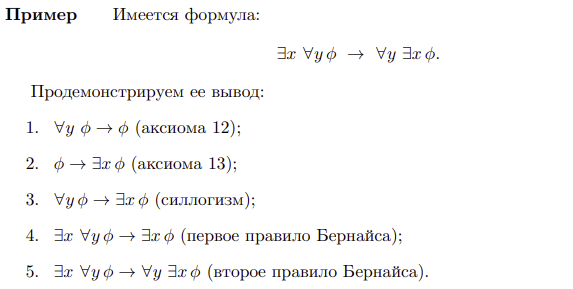
\includegraphics[width=0.7\linewidth]{images/1_definitions_sillog.png}

\subsection{Аксиомы равенства.}
\textbf{Определение:} Пусть $\sigma$ — произвольная сигнатура. Аксиомами равенства в сигнатуре $\sigma$ будут формулы:
\begin{enumerate}
    \item $\forall x \;\; (x=x)$ -- аксиома рефлексивности,
    \item $\forall x \forall y \;\;  \big((x=y)\to(y=x)\big)$ -- аксиома симметричности,
    \item $\forall x \forall y \forall z\;\;  \big(\big((x=y)\land(y=z)\big)\to(x=z)\big)$ -- аксиома транзитивности,
\end{enumerate}

\noindent а также для каждого функционального символа сформулируем аксиому равенства, которая говорит, что его значение не меняется, если аргументы заменить на равные.

\textit{Пример:} Для двухместного функционального символа $f$: $$\forall x_1 \forall x_2 \forall y_1\forall y_2\;\; \big(\big((x_1=x_2)\land(y_1=y_2)\big)\to \big(f(x_1,y_1)=f(x_2,y_2)\big)\big)$$
\noindent Для предикатных символов аксиомы равенства говорят, что истинный предикат остается истинным, если заменить аргументы на равные.

\textbf{Определение:} Формальная арифметика -- это аксиоматическая теория, расширяющая исчисление предикатов с равенством.

\subsection{Теории, модели, нормальные модели.}
Рассмотрим сигнатуру $\sigma$.

\textbf{Определение:} Множество Г замкнутых формул в сигнатуре называется теорией.

\textbf{Определение:} Формула называется замкнутой, если множество ее параметров пусто. Иначе говоря, все переменные замкнутой формулы должны быть связаны кванторами.

\textit{Пример:} $P,\;\; \forall xR(x),\;\; \exists x \forall y P(x,y),\;\; \forall x Q(x)\to \neg(\forall x \exists y R(x,y))$

\textbf{Определение:} Интерпретация $M$ сигнатуры $\sigma$ называется моделью теории Г, если все формулы из Г истинны в $M$.

\textbf{Определение:} Интерпретация $M$ сигнатуры $\sigma$ называется нормальной, если предикат равенства интерпретируется как тождественное совпадение элементов носителя.

\textbf{Определение:} Интерпретация $M$ сигнатуры $\sigma$ называется нормальной моделью теории Г, если она нормальная и все формулы из Г истинны в $M$.

\subsection{Аксиомы арифметики Пеано.}
Стандартная интерпретация: $\mathbb{N}, \; S$ -- следующее число, $0, +, -, =$ понимаются как обычно.

Аксиомы связанные с порядком:
\begin{enumerate}
    \item $\nexists x \; Sx=0 $
    \item $\forall x \forall y \; (Sx=Sy \to x = y)$
    \item Принцип индукции: $(\phi(0)\land \forall x (\phi(x)\to\phi(Sx)))\to\forall x \phi(x) $
\end{enumerate}

Аксиомы, связанные с арифметическими действиями:
\begin{enumerate}
    \item $\forall x \; x+0=x$
    \item $\forall x \forall y \; x+Sy=S(x+y)$
    \item $\forall x \; x\cdot 0 = 0$
    \item $\forall x \forall y \; x\cdot Sy = x\cdot y + x$
\end{enumerate}

\textit{Пример:} Как вывести, что $2+2 = 4$? В нашем языке это означает, что $SS0+SS0=SSSS0$
\begin{enumerate}
    \item $\forall x \forall y \; x+Sy = S(x+y)$ -- аксиома
    \item $SS0+SS0 = S(SS0+S0)$ -- подстановка $x=SS0, \; y=S0$
    \item $SS0+S0 = S(SS0+0)$ -- подстановка $x=SS0, \; y=0$
    \item $\forall x \; x+0 = x$ -- аксиома
    \item $SS0 + 0 = SS0$ -- подстановка $x=SS0$
    \item $\forall x \forall y \; (x=y \to Sx = Sy)$ -- аксиома равенства
    \item $SS0+0 = SS0\to S(SS0 + 0)=SSS0$ -- подстановка $x=SS0+0,\; y=SS0$
    \item $S(SS0+0)=SSS0$ -- modus ponens
    \item $SS0 + S0 = SSS0$ -- по транзитивности
    \item $S(SS0+S0)=SSSS0$ -- подстановка $x=S(SS0+0), \; y=SSS0$
    \item $SS0 + SS0 = SSSS0$ -- по транзитивности c 2.
\end{enumerate}

\subsection{Совместность, непротиворечивость, полнота теории.}

\textbf{Определение:} Теория Г называется совместной, если все формулы из Г могут быть одновременно истинны в некоторой интерпретации.

\textit{Пример 1:} $\{p \to q,\; q\to p,\; p\land q\}$ -- совместно, так как все верны на $(1,1)$.

\textit{Пример 2:} $\{ \neg (p \to q),\; \neg (q\to p)\}$ -- несовместно, тк первая формула верна только на $(1,0)$, а вторая -- только на $(0,1)$.

\textbf{Утверждение 1:} Г$=\{\phi\}:$ Г совместно $\Leftrightarrow \phi$ выполнима

\textbf{Утверждение 2:} Г$=\{\phi_1,\ldots,\phi_n\}:$ Г совместно $\Leftrightarrow (\phi_1\land\ldots\land\phi_n)$ выполнима
\newline \par \textbf{Определение:} Теория Г называется противоречивой, если из нее выводится некоторая формула $\phi$ и ее отрицание $\neg\phi$, и непротиворечивой в противном случае.

\textbf{Определение:} Непротиворечивая теория Г называется полной (в данной сигнатуре), если для любой замкнутой формулы  этой сигнатуры либо Г $\vdash\phi$, либо Г $\vdash\neg\phi$.